%%% LaTeX Template: Two column article
%%%
%%% Source: http://www.howtotex.com/
%%% Feel free to distribute this template, but please keep to referal to http://www.howtotex.com/ here.
%%% Date: February 2011

%%% Preamble
\documentclass[	DIV=calc,%
							paper=a4,%
							fontsize=12pt,%
							onecolumn]{scrartcl}	 					% KOMA-article class

\usepackage{lipsum}													% Package to create dummy text
\usepackage[brazil]{babel}										% English language/hyphenation
\usepackage[protrusion=true,expansion=true]{microtype}				% Better typography
\usepackage{amsmath,amsfonts,amsthm}					% Math packages
\usepackage[pdftex]{graphicx}									% Enable pdflatex
\usepackage[svgnames]{xcolor}									% Enabling colors by their 'svgnames'
\usepackage[hang, small,labelfont=bf,up,textfont=it,up]{caption}	% Custom captions under/above floats
\usepackage{epstopdf}												% Converts .eps to .pdf
\usepackage{subfig}													% Subfigures
\usepackage{booktabs}												% Nicer tables
\usepackage{fix-cm}													% Custom fontsizes
\usepackage[utf8]{inputenc}
\usepackage[top=2.5cm, bottom=2.5cm, left=2.5cm, right=2.5cm]{geometry}
\usepackage[ddmmyyyy]{datetime}
\addto\captionsenglish{%
	\renewcommand\tablename{Tabela}
	\renewcommand\figurename{Figura}
} 
 

 
%%% Custom sectioning (sectsty package)
\usepackage{sectsty}													% Custom sectioning (see below)
\allsectionsfont{%															% Change font of al section commands
	\usefont{OT1}{phv}{b}{n}%										% bch-b-n: CharterBT-Bold font
	}

\sectionfont{%																% Change font of \section command
	\usefont{OT1}{phv}{b}{n}%										% bch-b-n: CharterBT-Bold font
	}



%%% Headers and footers
\usepackage{fancyhdr}												% Needed to define custom headers/footers
	\pagestyle{fancy}														% Enabling the custom headers/footers
\usepackage{lastpage}	

% Header (empty)
\lhead{}
\chead{}
\rhead{}
% Footer (you may change this to your own needs)

%% ====================================
%% ====================================
%% mude o rodape  do projeto
%% ====================================
%% ====================================

\lfoot{\footnotesize \texttt{Template para entrega de texto} \textbullet ~Modelo de projeto}


\cfoot{}
\rfoot{\footnotesize página \thepage\ de \pageref{LastPage}}	% "Page 1 of 2"
\renewcommand{\headrulewidth}{0.0pt}
\renewcommand{\footrulewidth}{0.4pt}



%%% Creating an initial of the very first character of the content
\usepackage{lettrine}
\newcommand{\initial}[1]{%
     \lettrine[lines=3,lhang=0.3,nindent=0em]{
     				\color{DarkGoldenrod}
     				{\textsf{#1}}}{}}



%%% Title, author and date metadata
\usepackage{titling}															% For custom titles

\newcommand{\HorRule}{\color{DarkGoldenrod}%			% Creating a horizontal rule
									  	\rule{\linewidth}{1pt}%
										}

\pretitle{\vspace{-30pt} \begin{flushleft} \HorRule 
				\fontsize{50}{50} \usefont{OT1}{phv}{b}{n} \color{DarkRed} \selectfont 
				}

%% ====================================
%% ====================================
%% mude o titulo  do projeto
%% ====================================
%% ====================================

\title{Modelo de Processo Ágil Projeto X}					% Title of your article goes here

%% ====================================



\posttitle{\par\end{flushleft}\vskip 0.5em}

\preauthor{\begin{flushleft}
					\large \lineskip 0.5em \usefont{OT1}{phv}{b}{sl} \color{DarkRed}}
\author{Alexandre L'Erario, Breno Angelotti, Gabriel Romero, Jean Gonçalves, João Goulart, Mateus Merscher, Renan Batel }  	% Author name goes here


\postauthor{\footnotesize \usefont{OT1}{phv}{m}{sl} \color{Black} 
					\\Universidade Tecnológica Federal do Paraná - Câmpus Cornélio Procópio 								% Institution of author
					\par\end{flushleft}\HorRule}

\date{}																				% No date




%%% Begin document
\begin{document}
\maketitle
\thispagestyle{fancy} 	
\thispagestyle{empty}		% Enabling the custom headers/footers for the first page 
% The first character should be within \initial{}




%% ====================================
%% ====================================
%% mude o resumo  do projeto
%% ====================================
%% ====================================
\initial{E}\textbf{ste modelo de processo de software apresenta uma metologia de desenvolvimento ágil e cíclico para pequenos times de desenvolvimento com foco em projetos SaaS.}

%% ====================================
\begin{figure}
	\centering
	
\includegraphics{utfpr}
\end{figure}

\vspace{3cm}
\centerline{\textit{\textbf{\today}}}

\clearpage
    \renewcommand*\listfigurename{Lista de figuras}
\listoffigures

\renewcommand*\listtablename{Lista de tabelas}
\listoftables




\clearpage
\renewcommand{\contentsname}{Sumário}
\tableofcontents
\clearpage

%% ====================================
%% ====================================
%% Inicio do texto
%% ====================================
%% ====================================
\section{Introdução}
O modelo de processo de software apresentado neste documento é de estrutura ágil para equipes pequenas com projetos de empresas que tenham Software as a Service (SaaS). A proposta desse modelo é a autonomia do time de desenvolvimento e a visibilidade que cada desenvolvedor tem dentro do projeto, tudo isso contido dentro de um ciclo de desenvolvimento rápido e eficaz.

\begin{itemize}
	\item Projeto X (Definir nome);
	\item Integrantes: Breno Angelotti; Gabriel Romero; Jean Carlos Gonçalves; João Victor Goulart de Almeida; Mateus Merscher; Renan Batel.
	\item Github: https://github.com/goulartt/template;
\end{itemize}


\section{Processo}
O modelo de processo de software desenvolvido é de categoria ágil com ciclo de vida cíclico. O foco desse processo é desenvolver de forma rápida, e dando autonomia para equipe de desenvolvimento, ideal para empresas que contenham SaaS e várias equipes pequenas (squads) de desenvolvimento.

\subsection{Fases}

\subsection{Papéis}
O ideal para utilização desse modelo é uma equipe de 5 a 7 pessoas, sendo que toda equipe deve conter um Customer (cliente), um Agile Coach, um Product Owner, uma equipe de desenvolvimento e um Line Manager (Opcional), cuja suas respectivas funções são: 
\begin{itemize}
	\item \textbf{Customer}: Aquele que irá ditar o que será entregue.
	\item \textbf{Agile Coach}: Ajuda a manter o fluxo de trabalho, facilitando as retrospectivas, as reuniões de planejamento do ciclo, organizar a equipe de desenvolvimento e garantir a entrega prevista do ciclo. 
	
	\item \textbf{Product Owner}: Responsável pelo backlog e define prioridades das histórias, se comunicando diretamente com os stakeholders e apresentar ao cliente o andar do desenvolvimento do software. 
	
	\item \textbf{Squad}: Desenvolvedores responsáveis por um conjunto de funcionalidades. 
	
	\item \textbf{Line Manager}: responsável por no máximo 5 squads, irá alinhar com as equipes o que está sendo feito, participará em algumas reuniões para acompanhamento do squad sem influenciar no processo. Responsável pelo coaching e desenvolvimento de carreira individual de cada membro dos squads. Acompanha reclamações e problemas para criar planos de ação que melhorem o processo. 
\end{itemize}

\subsection{Atividades}
Em atividades do processo relacionadas aos papeis temos: 
\begin{itemize}
	\item \textbf{Especificação de requisitos}: levantar os requisitos com o cliente (Product Owner); 
	
	\item \textbf{Construção da história}: criar as histórias baseadas nos requisitos (Product Owner);  
	
	\item \textbf{Definição de backlogs e prioridades}: montar o backlog e definir as prioridades dos itens (Product Owner); 
	
	\item \textbf{Manter fluxo}: manter o fluxo das sprints e ajudar equipe de desenvolvimento (Agile Coach); 
	
	\item \textbf{Planejamento de Sprint}: definição de itens e duração da sprint (Agile Coach e Squad); 
	
	\item \textbf{Implementação da Sprint}: desenvolver os itens da sprint no tempo planejado (Squad); 
	
	\item \textbf{Correções}: tempo alocado da equipe para resolver casos emergenciais não previstos (Squad); 
	
	\item \textbf{Criação dos casos de teste}: os casos de teste são especificados e registrados de forma rastreável aos requisitos e então são agrupados de acordo com cada função. (Squad) 
	
	\item \textbf{Construção dos testes}: os scripts de automação são criados; (Squad) 
	
	\item \textbf{Execução dos testes}: os testes são executados nos ambientes necessários; (Squad) 
	
	\item \textbf{Validação}: os resultados dos testes são analisados e o pacote é enviado para release caso não haja falhas; (Squad) 
	
	\item \textbf{Documentação dos artefatos}: os artefatos da sprint são registrados (P.O, Agile Coach, Squad); 
	
	\item \textbf{Versionamento}: os artefatos são versionados (P.O, Agile Coach, Squad); 
	
	\item \textbf{Implantação}: o pacote é enviado para produção, se necessário (Squad); 
	
	\item \textbf{Análise e priorização da manutenção}: o relatório de registro de erros é analisado e as ações/correções são priorizadas (Agile Coach); 
\end{itemize}

\subsection{Disciplinas}

\subsection{Artefatos}

\subsection{Guidance}

\subsection{Interações}

\subsection{Iterações}

\subsection{Milestones}

\subsection{Ferramentas}

\subsection{Feedback}

\section{Execução do projeto}

Relacione as atividades com os integrantes, crie um cronograma conformed orientações
\subsection{Backlog e sprints}
-- item obrigatório --

Evidencie todos os stakeholders involvidos


\subsection{Estado atual}
Apresente os artefatos gerados em ordem cronológica, conforme processo.

\clearpage
\section{Referências Bibliograficas}
\begingroup
\renewcommand{\section}[2]{}
Utilize o mendley, o jabref ou diretamente o bibtex para gerenciar suas referências biliográficas. As referências são criadas automaticamente de acordo com o uso no texto.

Exemplo: Redes de computadores, segundo \cite{scrumguide} é considerada..... Já \cite{leia77} apresenta uma versão...

Analisando os pressupostos de \cite{Buerger1989} e \cite{leia77} concluimos que....

\bibliographystyle{ieeetr}
\bibliography{referencias/referencias} 
\endgroup



\section{Elementos textuais - Alguns exemplos}

Esta seção apresenta exemplos de elementos textuais. \textbf{Remova-a da versão final do texto}.


\subsection{Colocar elementos em itens}

Texto antes da lista

\begin{itemize}
	\item First item in a list 
	\item Second item in a list 
	\item Third item in a list
\end{itemize}

\subsubsection{Uma subseção de terceiro nivel}

Exemplo de uma subseção

\subsection{Tabelas}

Utilize o site http://www.tablesgenerator.com/ para elaborar as tabelas de seu trabalho.
Para adicionar uma tabela utilize: a tag input, passando o arquivo da tabela como parametro

\begin{table}[h!] % coloque h! para forcar a posicao
\centering
\caption{Modifique a legenda e crie um label}
\label{tab2} %com este label vc faz referencia no texto
\begin{tabular}{|l|l|l|l|l|}
\hline
\multicolumn{1}{|c|}{\textbf{Este é um exemplo de tabela}} & \multicolumn{2}{c|}{\textbf{C1}} & \multicolumn{2}{c|}{\textbf{C2}} \\ \hline
Você pode criar a tabela no excel                          & 1              & 2               & 3               & 4              \\ \hline
Exportar para CSV                                          & 5              & 6               & 7               & 8              \\ \hline
E importar no Table Generator                              & 9              & 10              &                 &                \\ \hline
\multicolumn{5}{|c|}{\textit{Gere o tex, e adicione em seu arquivo}}                                                             \\ \hline
\end{tabular}
\end{table}

Dentro do arquivo você deve definir o label e pode utilizá-lo para referenciar. Exemplo:
Na tab \ref{tab2} temos a relação de ....


Você também pode modificar a tabela manualmente, incluindo, por exemplo h! dentro de sua definição. Veja no exemplo tab2.tex

\subsection{Figuras}

As figuras podem ser no formato PDF, JPG, PNG. Você pode referenciá-las da mesma maneira que tabelas. Exemplo: A figura \ref{fig1} apresenta.....

Não se preocupe o local em que a figura será renderizada em seu texto. Preocupe-se em criar referência para ela, ou seja, toda figura e tabela deve conter pelo menos uma referência no texto.

\begin{figure}
\centering
\includegraphics[width=\textwidth]{fig1}
\caption{Exemplo de figura com escala horizontal}
\label{fig1}
\end{figure}


\begin{figure}
	\centering
	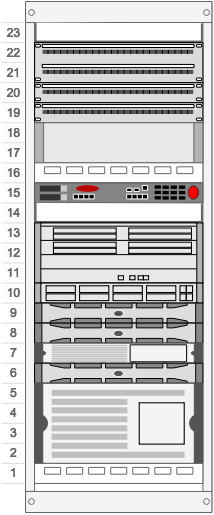
\includegraphics[]{fig2}
	\caption{Exemplo de figura sem escala}
	\label{fig2}
\end{figure}

Você pode rotacionar figuras também. Para isso utilize o parâmetro angle=-90. Repare que a escala da figura foi modificada pelo parametro height. Você também pode utilizar scale

\begin{figure}
	\centering
	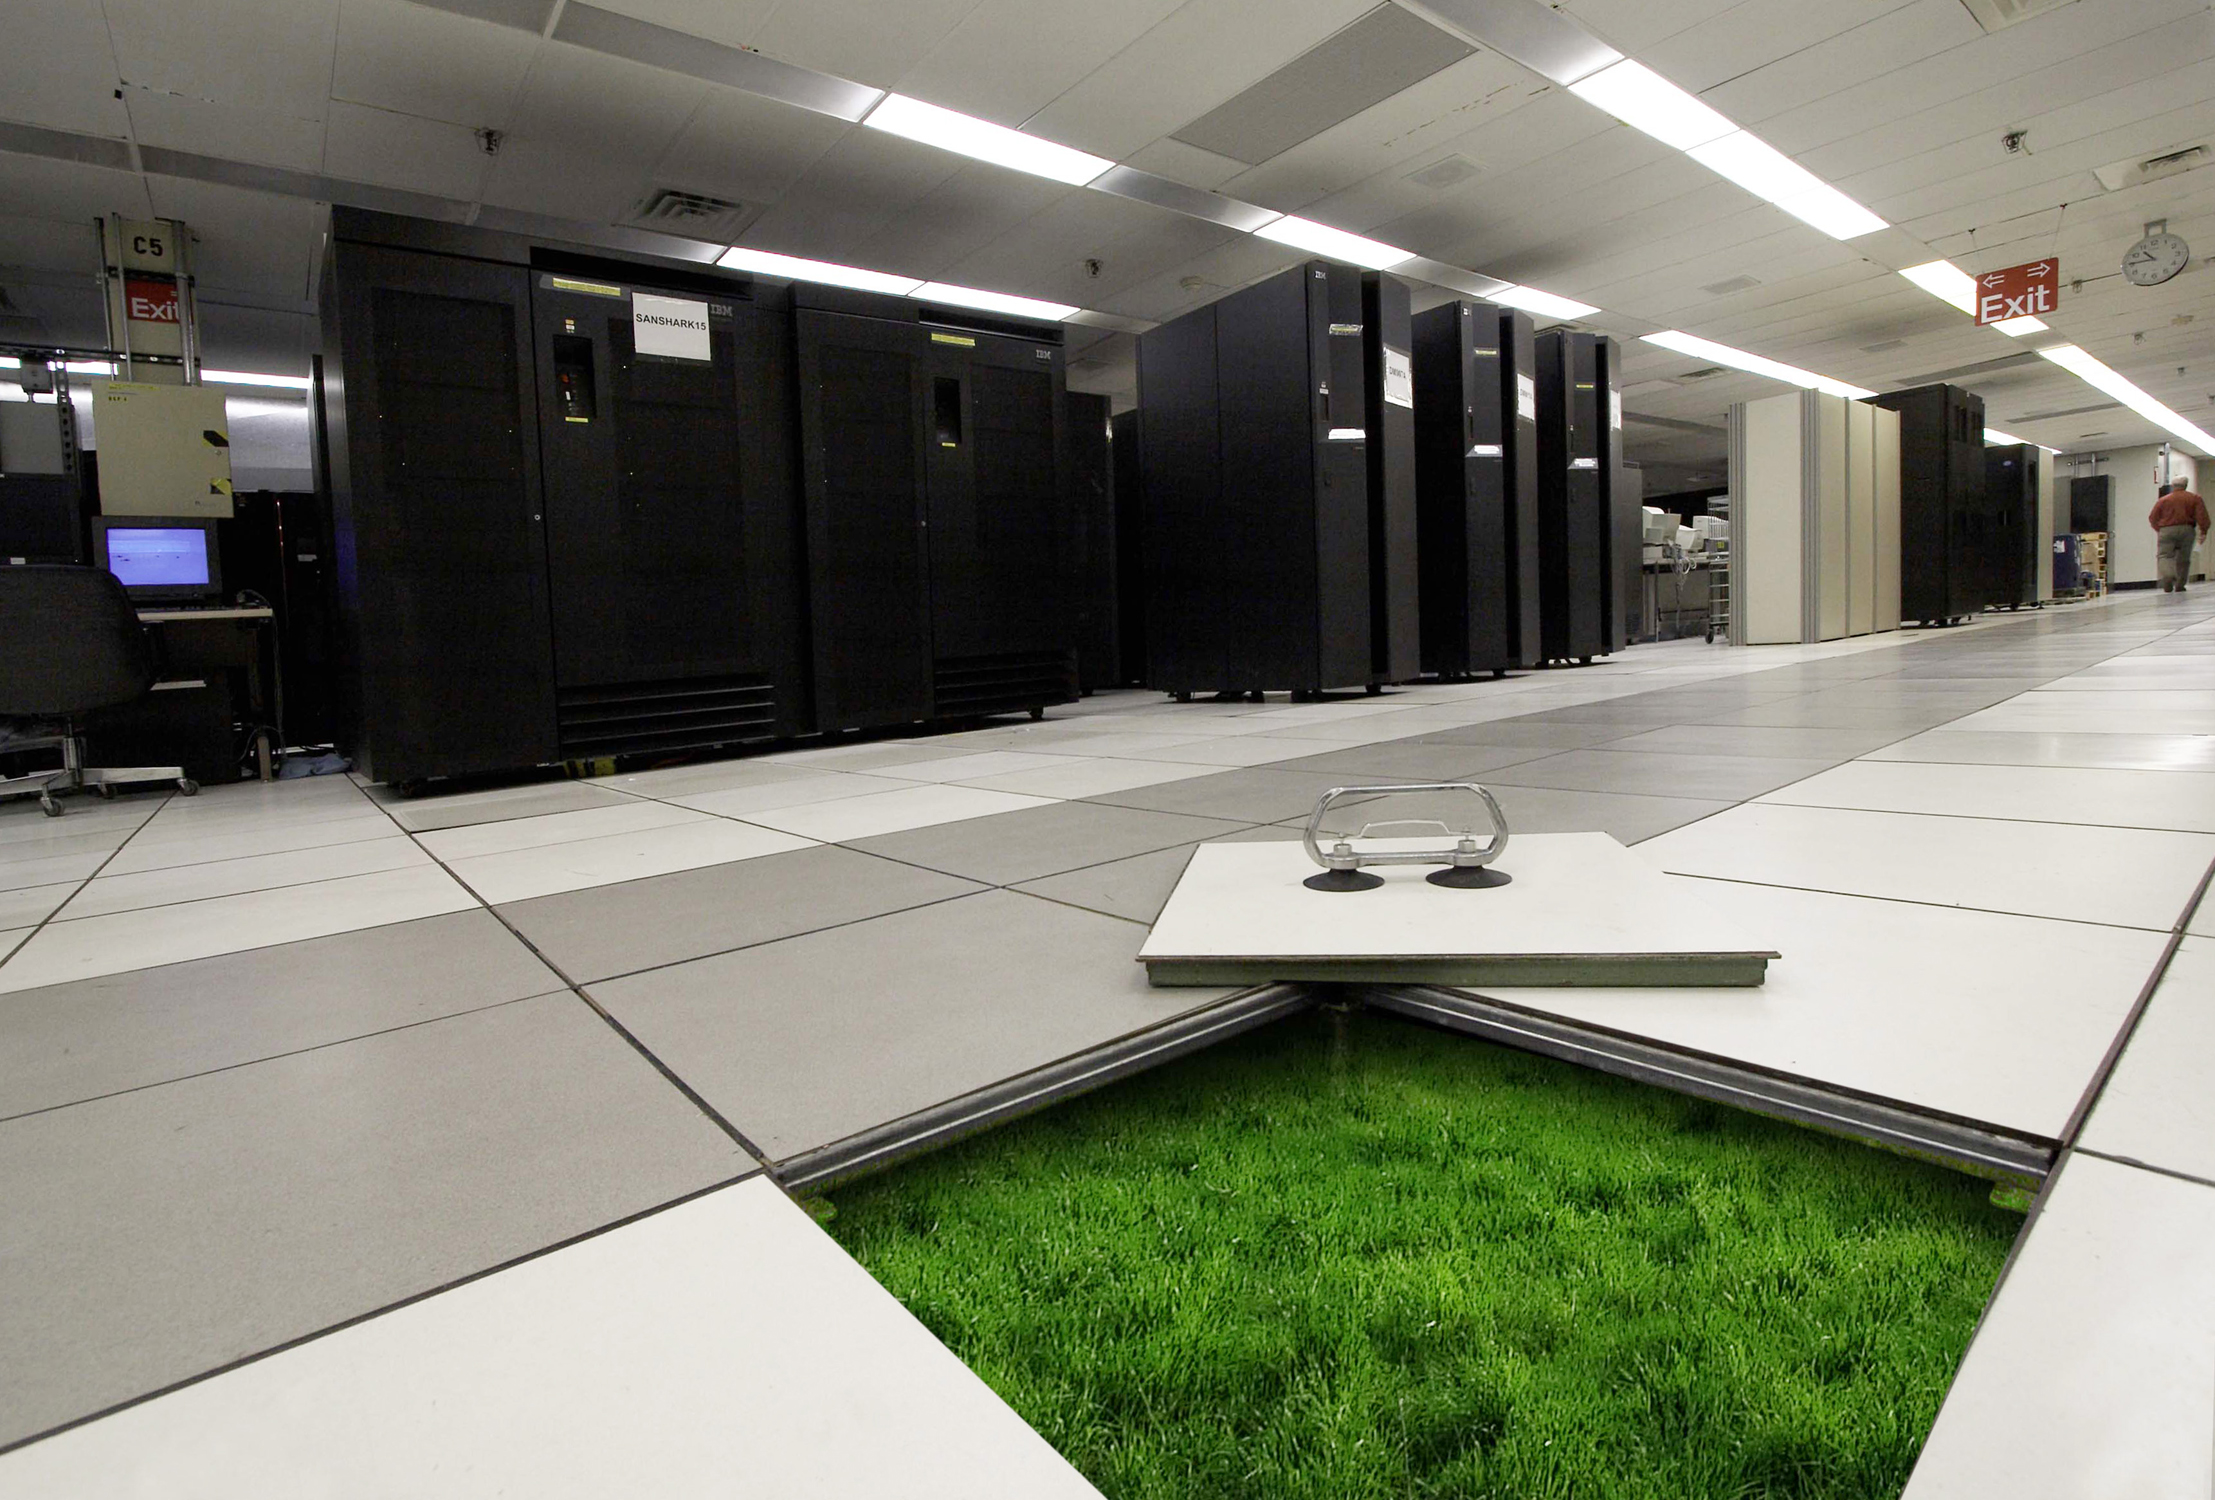
\includegraphics[height=\textwidth,angle=-90]{fig3}
	\caption{Exemplo de figura rotacionada}
	\label{fig3}
\end{figure}


%% ***********************************************************************
%% === ate aqui    =====  ================================================
%% ***********************************************************************

\end{document}